\section{Idée générale}

Les bases de données fédérées ont pour but de proposer une vue unique à un ensemble de bases de données de diverses natures. Ces bases de données peuvent être séparées géographiquement. L’utilisateur consulte ainsi les données soumises un modèle unifié et cohérent.

Cette problématique intervient particulièrement lors de la fusion de systèmes d’information, voire d’entreprises, lorsqu’on souhaite associer des bases de données différentes sans pour autant les regrouper dans une base unique et homogène, ce qui aurait un coût très important.

L’accès aux données et leurs mises à jour se font via un langage unique, ce qui donne une certaine transparence, puisque l’utilisateur ne se préoccupe pas de savoir dans quelles bases se trouvent les données qu’il souhaite et quel est le langage à appliquer pour les récupérer.

La base de données fédérée se doit aussi d’être extensible, afin de permettre l’intégration de nouvelles bases, possiblement utilisant encore une technologie différente. De plus, chaque base est rendue autonome, ce qui va dans le sens de l’extensibilité. Enfin, la base de données fédérées est avant tout une base de données, et doit remplir son rôle en gardant en tête les contraintes de performances, aspect important des bases de données.

Pour finir, gardons à l’esprit l’existence possible de conflits, de par la nature même des bases de données fédérées. Ces conflits, directement liés à l’hétérogénéité des différentes bases fédérées, se doivent d’être identifiés et gérés lors de la procédure de fédération. C’est aussi ce genre de difficulté que ce projet nous permettra d’appréhender plus facilement à l’avenir.


\section{Fonctionnement avec une requête simple}

Afin d’appréhender le fonctionnement général d’une base de données fédérée, étudions le parcours d’une requête simple. Cette requête est émise par l’utilisateur en XQuery et prend la forme suivante :

\begin{verbatim}
for $nom in doc()//nom

where $nom/..//age > 18

return $nom
\end{verbatim}

Supposons la base de données fédérée comme composée de deux bases : l’une qu’on appellera R1 est une base de données SQL et contient deux colonnes “id” et “nom”, l’autre appelée R2 est une base de données XML et contient des “personnes” possédant un élément “id” et un élément “age”. 

\begin{figure}[h!]
    \centering
    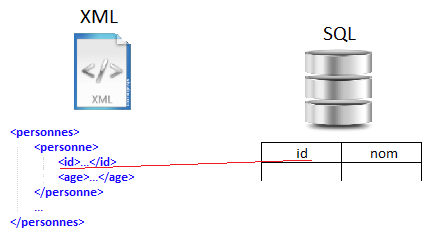
\includegraphics[width=0.8\textwidth]{ressources/graphiques/xmlAndSql_simple_example.png}
    \caption{Exemple simplifié d'une base fédéré}
\end{figure}


Avec cette requête, l’utilisateur cherche à accéder au nom des personnes présentes dans la base fédérée étant majeures. Elle est effectuée en accord avec un schéma fédéré, qui est défini pour représenter la structure virtuelle de la base de données vue par l’utilisateur.

La requête est transmise au médiateur, élément central de l’architecture fédérée. Pour commencer, le médiateur fait vérifier l’intégrité et le bon format de cette requête par le module verifier. Si ce module n’accepte pas la requête, elle est abandonnée. Sinon, il va diviser la requête, via son module splitter dans le but d’adresser les sous-requêtes aux bonnes bases de données. Dans notre cas, on aura une sous-requête sur R2 demandant la liste des “id” dont “age” est supérieur à 18, et une sous-requête sur R1 qui rendra la liste des “noms” dont les “id” ont été rendus par la première sous-requête. Mais avant d’être émises, ces sous-requêtes seront traduites dans un langage pivot.

Ces sous-requêtes traduites sont transmises aux différents wrappers chargés de chaque base de données concernée. Le wrapper W2 reçoit la requête qui concernera R2 et la traduit donc en XQuery afin d’interroger R2. Il capte ensuite la réponse de R2, la traduit et l’envoie au médiateur. De même W1 traduira, cette fois-ci en SQL, et transmettra la réponse traduite au médiateur.

C’est cette fois-ci le module merger du médiateur qui entre en jeu et remplit son rôle de fusion des réponses des différentes sous-requêtes dans le but de répondre à la requête initiale.

Enfin, un helper pourra intervenir en sortie du médiateur pour traduire la réponse dans le langage souhaité.

\section{Les bases de données fédérées}

\subsection{Couplage de bases de données}

Il existe deux grands types de bases de données fédérées : les bases faiblement couplées et les bases fortement couplées. Nous nous sommes intéressés pour ce projet aux bases de données fédérées faiblement couplées

En effet, les bases fortement couplées sont constituées d’un ensemble de bases ayant accès à toutes les autres bases. Chaque base fédérée est chargée de s’occuper de l’interfaçage avec les autres bases. Pour N base fédérées, chaque base doit implémentées N - 1 interfaces, ce qui représente au total N(N-1)/2 interfaces au totales. Nous avons donc choisi d’étudier l’autre modèle qui apporte plus de flexibilité. Dans la suite nous traiterons uniquement du cas faiblement couplé.

L’idée générale de ce modèle est de regrouper sous un modèle unique des bases de données hétérogènes. L’architecture est consituée de couches d’abstraction successives. Les données qui passent à travers les couches sont transformées de manière à découpler la représentation des données de leur stockage physique.

Les données sont transmises à travers un certain nombre de couches. Ces couches communiquent entre elles grâce à un langage intermédiaire de haut niveau. Chaque couche possède une représentation des données de la base qui lui sont propres, et est constituée de composants appellés “wrappers”. La couche la plus basse se charge de l’interfaçage des sources avec la fédération.

Nous utilisons des schémas pour qualifier ces représentations des données propres à chaque couches. Nous utilisons quatre niveaux dans notre étude :

\begin{itemize}
    \item Le schéma externe : la représentation des données manipulée par l’utilisateur ;

    \item Le schéma fédéré : la représentation interne des données agrégées ;

    \item Le schéma composant : la représentation des données communiquée aux sources ;

    \item Le schéma local : la représentation des données dans les sources.
\end{itemize}

\subsection{Problèmes communs liés aux architectures fédérées}

La fédération de sources différentes ou distantes pose naturellement des difficultés récurrentes. A partir de l’ouvrage \textit{Database Systems}\cite{bib:dbsys}, nous avons cherché à étudier et appréhender les problèmes liés à l’architecture fédérée. Ces problèmes peuvent provenir directement des situations suivantes :

\begin{itemize}
    \item hétérogénéité de la communication : différents systèmes reposent généralement sur différents protocoles de communication et ces différents protocoles sont à traiter indépendemment les uns des autres ;
    \item hétérogénéité des langages de requête : différents systèmes emploient différents langages de requêtes, ces langages sont en particulier variable selon le type des bases considérées, par exemple XQuery pour XML ou Cypher pour Neo4j ;
    \item hétérogénéité des schémas : différents types de données peuvent être représentés de manières différentes, par exemple un objet comportant d’autres sous-objets pourra être représenté par des balises internes en XML et par des références vers des tables (clefs étrangères) en SQL ;
    \item  hétérogénéité des types : des données peuvent parfois être représentées par des types différents selon l’implémentation, par exemple un numéro de téléphone peut être vu comme un entier ou une chaîne de caractères ;
    \item hétérogénéité sémantique : certaines données peuvent être regroupées dans différentes catégories sémantiques, exemple une première base peut considérer un personnage comme un “adjuvant” ou une autre comme un “humain”.
\end{itemize}

Cependant, ces problèmes sont généralement traités par l’architecture même de la fédération. En effet, on pourra résoudre les problèmes liés à l’hétérogénéité de communication ou de langages de requêtes grâce à point d’accès unique vers la base. L’hétérogénéité des schémas est masquée par des étapes successives de transformation et la représentation interne. Enfin, l’hétérogénéité des types peut être gommée dans les couches basses de la fédération, notamment par l’action des wrappers.


